% --------------------------------------------
% Author: Felipe Alfonso González
% License: MIT
%
%%%%%%%%%%%%%%%%%%%%%%%%%%%%%%%%%%%%%%%%%

%----------------------------------------------------------------------------------------
%	PACKAGES AND OTHER DOCUMENT CONFIGURATIONS
%----------------------------------------------------------------------------------------

\documentclass[
    a4paper, % Paper size, use either a4paper or letterpaper
    10pt, % Default font size, can also use 11pt or 12pt, although this is not recommended
    unnumberedsections, % Comment to enable section numbering
    twoside, % Two side traditional mode where headers and footers change between odd and even pages, comment this option to make them fixed
]{LTJournalArticle}

\usepackage{amsmath}

\usepackage{hyperref}

\addbibresource{biblio.bib} % BibLaTeX bibliography file

\runninghead{} % Leave this command empty for no running head

\footertext{} % Leave this command empty for no footer text

\setcounter{page}{1} % The page number of the first page, set this to a higher number if the article is to be part of an issue or larger work

\usepackage{amsmath} % Add this line to load the amsmath package

\usepackage{graphicx}

%----------------------------------------------------------------------------------------
%	TITLE SECTION
%----------------------------------------------------------------------------------------

\title{Big Data en Marketing}

% Authors are listed in a comma-separated list with superscript numbers indicating affiliations
% \thanks{} is used for any text that should be placed in a footnote on the first page, such as the corresponding author's email, journal acceptance dates, a copyright/license notice, keywords, etc
\author{%
    Felipe Alfonso González\textsuperscript{1}\thanks{Corresponding author: \href{mailto:f.alfonso@res-ear.ch}{f.alfonso@res-ear.ch}}\\
    \textit{ Computer Science Engineer}\\
    \footnotesize Institute of Arts and Communication Sciences (IACC), Chile\\[-6pt]
    \footnotesize Candidate for Master in Big Data, ENEB / Isabel I University\\[-6pt]
    \footnotesize\href{mailto:f.alfonso@res-ear.ch}{f.alfonso@res-ear.ch} - 
    \href{https://glzengrg.com}{glzengrg.com} - 
    Twitter: \href{https://twitter.com/felipealfonsog}{@felipealfonsog} - 
    LinkedIn: \href{https://linkedin.com/in/felipealfonsog}{felipealfonsog}\\
    \scriptsize This manuscript has been authored using the typesetting system \LaTeX{}. \\[-6pt]
    \scriptsize This manuscript is released under the BSD 3-clause License. \\
}




% Full-width abstract
\renewcommand{\maketitlehookd}{%
    \begin{abstract}
        \noindent En el entorno altamente competitivo actual, la retención y satisfacción de clientes son imperativos fundamentales. A lo largo de la historia del marketing, se han implementado diversas estrategias para impulsar las ventas y fomentar la lealtad, pero en la actualidad, la personalización se ha vuelto esencial en este contexto de feroz competencia. 
        Este paper explora el marketing desde la perspectiva del big data, destacando cómo las empresas pueden aprovechar los datos disponibles sobre clientes y entorno para diseñar estrategias altamente personalizadas. Ya no es suficiente con promociones genéricas; ahora, la clave radica en ofertas específicas que se alineen con las preferencias individuales de cada cliente. 
        Al reconocer que los clientes son la piedra angular de una empresa, se enfatiza la importancia de planificar acciones y estrategias personalizadas. Estos enfoques no solo aseguran la supervivencia de la empresa en un mercado dinámico, sino que también generan lealtad y fidelidad del cliente, aportando un valor significativo al negocio. 
        
    \end{abstract}
}

%----------------------------------------------------------------------------------------



\begin{document}

\maketitle % Output the title section

%----------------------------------------------------------------------------------------
%    ARTICLE CONTENTS
%----------------------------------------------------------------------------------------

\section{Introduction}

En el panorama empresarial actual, marcado por una competencia feroz, la retención de clientes y su satisfacción plena se presentan como objetivos cruciales para la supervivencia y el éxito de cualquier empresa. A lo largo de la historia, el marketing ha evolucionado desde estrategias generales hasta reconocer la necesidad de personalización en un mundo donde cada cliente es único. Este paper aborda el desafío de implementar estrategias de marketing desde la perspectiva del big data, explorando cómo la información sobre clientes y su entorno puede ser aprovechada para diseñar ofertas altamente específicas. En un contexto donde los clientes son la esencia misma de la empresa, este enfoque personalizado no solo asegura la permanencia en el mercado, sino que también cultiva la lealtad y la conexión duradera con la clientela, generando un valor distintivo para el negocio. \cite{ENEB2023}.

\subsection{El Marketing: necesidades, deseos y demandas}

%%% Necesidades, deseos, demandas 
Todas las personas pueden tener diferentes tipos de necesidades, que son parte de la esencia humana y pueden ser físicas (como alimentarse), seguridad, o sociales o individuales; pero sus deseos pueden estar alineados con sus necesidades, que pueden ser físicas, como alimentarse o sentirse seguro, o algún tipo de realización personal, entre otras. Pueden variedad según incluso por cuan importantes deseas sentirse. En relación a las demandas, son los deseos, y estas se convierten en demanda cuando existe esa capacidad adquisitiva. 

%%% Productos o Servicios
El ser humano, satisfaces sus necesidades con productos y servicios. Pueden ser estos intangibles como los servicios en algún área, o tangibles. Pueden ser susceptibles a algo que puede ser ofrecido para satisfacer necesidades y deseos. 

%%% Valor coste y satisfacción
 Todos los consumidores toman decisiones basadas en expectativas que les plantean las diferentes ofertas. Las expectativas de valor que les plantean en las diferentes ofertas. 
 
Los consumidores eligen productos según las expectativas netas de valor, la diferencia entre aspectos positivos y negativos esperados. Este valor impacta en la satisfacción del cliente y su comportamiento futuro, al comparar expectativas con la experiencia real de compra.

El marketing surge del intercambio, un proceso donde las personas satisfacen necesidades a través de ofrecer algo a cambio de dinero, bienes o servicios. Para que el intercambio ocurra, deben existir al menos dos partes con algo de valor para la otra, capacidad de comunicación, libertad de aceptar o rechazar la oferta, y la creencia de que es apropiado tratar con la otra parte. El intercambio es un proceso continuo, y cuando se llega a un acuerdo, se denomina transacción. El marketing de relaciones busca construir relaciones duraderas basadas en confianza mediante la entrega consistente de productos de calidad, buen servicio y precios razonables.


Un mercado es el conjunto de consumidores que comparten una necesidad o deseo y están dispuestos a intercambiar elementos de valor. Su tamaño depende del número de personas con la necesidad específica, recursos atractivos para otros, y la disposición de intercambiar.

El marketing se centra en actividades relacionadas con los mercados para facilitar intercambios potenciales que satisfacen necesidades y deseos. En este proceso, participan dos partes: el buscador de intercambios, usualmente una empresa compitiendo en un mercado, y el receptor. La eficacia del buscador se ve afectada por factores del entorno como demografía, economía, tecnología y aspectos socio-culturales.

%%  Inserting image 
\begin{figure}[h]
  \centering
  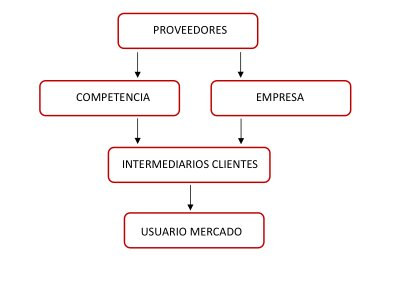
\includegraphics[width=0.7\linewidth]{./images/graph-mkt.jpg}
  \caption{Partes que confirman el marketing}
  \label{fig:etiqueta}
\end{figure}
%% End insert image 




\subsection{Gestión del marketing}

La gestión de marketing implica planificar y ejecutar estrategias para productos, precios, promoción y distribución. Se centra en la gestión de la demanda, ajustando la oferta a las cambiantes condiciones del mercado. La retención de clientes es esencial, dada la alta inversión en la adquisición de nuevos clientes y el riesgo de repercusiones negativas en redes sociales. Las orientaciones empresariales, como producción, producto, ventas, marketing y marketing social, reflejan filosofías distintas que impactan las estrategias de marketing. En resumen, la gestión de marketing es un proceso dinámico que busca no solo intercambios, sino también relaciones a largo plazo con los clientes.


%% Enfoque de producción - pp. 8


















%------------------------------------------------

\section{Methodologies}

To discern the effectiveness of code challenges and explore alternative assessment methods, a thorough analysis of existing literature, industry practices, and case studies was conducted. The goal was to elucidate the correlation between success in code \section{Redefining Engineering Excellence}

Engineering is an amalgamation of cognitive agility, problem-solving acumen, and interpersonal skills. An engineer's worth lies not in the mastery of a predefined set of skills, but in their ability to learn, collaborate, and innovate. By championing these traits, organizations foster a culture of resilience and evolution.

\section{Promoting a Paradigm Shift}

A transformative shift in assessment paradigms is overdue. Code challenges, while valuable, should be complemented with broader evaluations. Organizations stand to gain by emphasizing holistic attributes such as adaptability, critical thinking, and collaboration. The engineering landscape beckons for engineers who can not only code, but also envision, communicate, and innovate.

%------------------------------------------------

\section{Conclusion}

This paper challenges the prevailing narrative that engineers must possess exhaustive knowledge and underscores the limitations of code challenges. It advocates for an inclusive assessment approach that values problem-solving, adaptability, and teamwork. Engineering is an ever-evolving discipline, necessitating engineers who can navigate complexities and contribute meaningfully to the collaborative process \cite{Smith2020,Johnson2019,Brown2021,Garcia2022}.

%----------------------------------------------------------------------------------------
%    REFERENCES
%----------------------------------------------------------------------------------------

\printbibliography % Output the bibliography

%----------------------------------------------------------------------------------------

\end{document}
